% Two-column layout approximating the USENIX 2019 (v3) template used by SOUPS:
% US letter, 10pt Times, 7in x 9in text block, 0.33in column gap.
\documentclass[letterpaper,twocolumn,10pt]{article}
\usepackage[utf8]{inputenc}
\usepackage[T1]{fontenc}
\usepackage{mathptmx}
\usepackage[textwidth=7in,textheight=9in,top=1in,columnsep=0.33in,headsep=0pt,headheight=0pt]{geometry}
\usepackage{graphicx,booktabs,tabularx,array,amsmath,amssymb,newunicodechar,microtype,enumitem,xurl}
\usepackage[hidelinks]{hyperref}
\usepackage[font=small,labelfont=bf,labelsep=colon,skip=4pt]{caption}
\usepackage{titlesec}
\titleformat{\section}{\normalfont\large\bfseries}{\thesection}{1em}{}
\titleformat{\subsection}{\normalfont\normalsize\bfseries}{\thesubsection}{1em}{}
\titleformat{\subsubsection}{\normalfont\normalsize\bfseries}{\thesubsubsection}{1em}{}
\titlespacing*{\section}{0pt}{10pt}{5pt}
\titlespacing*{\subsection}{0pt}{8pt}{4pt}
\titlespacing*{\subsubsection}{0pt}{6pt}{3pt}
\setlist{nosep,leftmargin=*}
\newunicodechar{ρ}{\ensuremath{\rho}}
\newunicodechar{φ}{\ensuremath{\phi}}
\newunicodechar{β}{\ensuremath{\beta}}
\newunicodechar{−}{\ensuremath{-}}
\newunicodechar{≤}{\ensuremath{\leq}}
\newunicodechar{×}{\ensuremath{\times}}
\newunicodechar{→}{\ensuremath{\rightarrow}}
\providecommand{\tightlist}{\setlength{\itemsep}{0pt}\setlength{\parskip}{0pt}}
\renewcommand{\topfraction}{0.9}\renewcommand{\dbltopfraction}{0.9}\renewcommand{\textfraction}{0.07}\renewcommand{\floatpagefraction}{0.75}\renewcommand{\dblfloatpagefraction}{0.75}\setcounter{topnumber}{3}\setcounter{dbltopnumber}{3}
\pagestyle{empty}
\date{}
\title{\Large\bfseries Why Passkey Implementations Diverge: Root Causes, Harms, and\\Guideline Gaps Across 111 Websites}
\author{Arnav Goel \qquad Neeraj Yadav \qquad Dev Singh Shekhawat\\\relax {\normalsize Department of Computer Science and Engineering, Shiv Nadar University}}
\begin{document}
\maketitle
\thispagestyle{empty}
\subsection*{Abstract}
Passkeys follow one set of standards, yet websites implement them differently. A recent SOUPS study measured these differences across 111 websites using 28 comparison factors, but did not explain why they arise. We conducted a secondary analysis of that study's per-site data, combined with a structured coding of five guidance sources: the FIDO Alliance Design Guidelines, WebAuthn Level 3, and Google, Apple and Microsoft developer guidance. Factors on which guidance sources agree are implemented more consistently (Spearman ρ = −0.45, p = 0.016, with FIDO weighted at 70\%), and the effect is robust to removing duplicate factors, browser-default factors or any single source, and to weighting all sources equally. One of the three reported website clusters is largely a single registration choice counted four times, concentrated in e-commerce and finance. The most harmful gap is unguided: 65\% of websites re-authenticate users neither before a passkey is added nor before one is deleted. For the 21 factors that have not converged, guideline problems are the most likely main cause for 8, with the rest explained by technical defaults, legacy architecture, deliberate risk decisions and measurement artefacts. We propose 10 changes to the FIDO guidelines, 9 practices for websites and 4 requests to platform vendors, led by a lifecycle-security pattern and normative, versioned guidance.

\section{Introduction}

Passkeys are a phishing-resistant replacement for passwords built on the FIDO2 and WebAuthn standards {[}3, 4{]}. Because every website relies on the same underlying protocol, users might expect the passkey experience to be similar from one site to the next. It is not. Ramat et al.~{[}1{]} evaluated 111 websites against 28 comparison factors and found that core passkey support is converging while supporting features remain uneven. Only 36\% of websites place passkeys above passwords, 42\% offer passkey autofill, 3\% offer a passkey during account recovery, and roughly 70\% do not re-authenticate users when a passkey is added or removed. Inconsistency of this kind matters because users carry expectations from one website to another {[}19{]}, and because some of the missing features protect accounts.

The original study was descriptive by design. Its authors note that their distance measure ``does not clarify why websites differ or identify which specific design choices are most responsible for those differences'' {[}1{]}. Answering that question determines who should act. If an inconsistency stems from vague guidance, the FIDO Alliance should revise its text. If it stems from browser behaviour, platform vendors must act. If it reflects a legitimate risk decision, forcing uniformity would be a mistake. If it is an artefact of the rubric, the measurement should change.

To address this gap, we structured our analysis around four research questions. \textbf{RQ1:} How strongly and how consistently do current guidance sources address each of the 28 factors? \textbf{RQ2:} Does the strength or agreement of guidance explain which factors are implemented consistently? \textbf{RQ3:} What is the most likely cause of each remaining inconsistency, and which inconsistencies cause meaningful usability or security harm? \textbf{RQ4:} What changes to guidelines, websites and platforms would reduce harmful inconsistency without restricting legitimate product decisions?

To answer these questions, we re-analysed the original study's published per-site scores and coded the current text of five guidance sources against every factor. We then tested hypotheses about each factor's cause using co-occurrence, site attributes and browser release timelines, and classified each factor by cause and by harm.

This study makes four main contributions. First, it provides a coded map of five guidance sources against all 28 factors, showing that the FIDO guidelines contain no normative MUST or SHOULD language and have not been updated since May 2024. Second, it provides statistical evidence, on the original study's own data, that agreement among guidance sources predicts implementation consistency. Third, it shows that a substantial part of the measured inconsistency comes from a single registration setting and from rubric artefacts, and it classifies every factor by its most likely cause and its harm. Finally, it offers 23 evidence-based recommendations for the FIDO Alliance, website developers and platform vendors.

\section{Background and Related Work}

A passkey is a discoverable FIDO2 credential that is either synchronised through a credential manager or bound to a single device such as a hardware security key (HSK) {[}3{]}. The relying party (RP) shapes the user experience through WebAuthn options {[}4{]}: \texttt{authenticatorAttachment} and \texttt{hints} restrict which authenticators may be used at registration, conditional mediation enables passkey autofill, and WebAuthn Level 3 adds conditional create for automatic passkey upgrades and the Signal API for keeping credential managers in sync with the server. These options are where an RP's implementation choices become visible differences.

\subsection{Comparative Evaluation and Consistency}

Comparative frameworks are a common way to evaluate authentication systems at scale. Lyastani et al.~{[}11{]} measured the consistency of two-factor authentication journeys on top-ranked websites and found substantial variation. Ramat et al.~{[}1{]} adapted this approach to passkeys, deriving 23 comparison factors deductively from the FIDO guidelines and 5 through open coding. They coded 111 websites from passkeys.directory as match, partial match or non-match between February 2025 and February 2026 on Windows 11 with Google Chrome, and grouped them by Euclidean distance and average-linkage clustering into Standard (n = 89), Selective (n = 20) and Experimental (n = 2) implementers. Our work builds directly on their data and asks why the differences they observed exist.

\subsection{Deployment Obstacles and Lifecycle Security}

Prior work suggests that differences in deployment have organisational and technical roots. Lassak et al.~{[}12{]} found that companies struggle with legacy systems, account recovery and uneven platform support when deploying FIDO2. Studies of account recovery {[}14, 15{]} show that fallback and recovery flows frequently undo the security of strong authenticators. Daffalla et al.~{[}13{]} analysed passkeys under interpersonal threat models and showed how temporary session access can be converted into persistent account control. Huaman et al.~{[}17{]} documented interaction problems between password managers and websites, a problem that reappears with passkeys as credentials orphaned in a credential manager after deletion on the website. Usability studies of FIDO2 {[}16{]} report generally positive perceptions but persistent confusion around device loss, fallback and multi-device use.

\subsection{Design Guidelines}

The FIDO Alliance Design Guidelines {[}3{]} organise passkey UX into required, optional and security-key patterns. The current text is hosted on Passkey Central, carries pattern dates of May 2022, May 2023 and May 2024, and has no version number or changelog. Google {[}5, 6{]}, Apple {[}7{]} and Microsoft {[}8{]} publish their own developer guidance, which sometimes extends and sometimes contradicts FIDO's. WebAuthn Level 3 {[}4{]} is the only source that uses RFC 2119 keywords, and it addresses protocol behaviour rather than interface design. Ramat et al.~used the June 2023 FIDO text as their baseline. To our knowledge, no prior work has linked observed passkey inconsistencies to the strength or agreement of the guidance behind each behaviour.

\section{Methodology}

We conducted a secondary, desk-based study in five stages, shown in Figure 1. We first reproduced the original dataset (Section 3.1), then coded current guidance against each factor (Section 3.2), measured each factor's inconsistency (Section 3.3), tested candidate explanations (Section 3.4), and classified each factor by cause and harm (Section 3.5). We collected no new website observations.

\begin{figure*}[t]\centering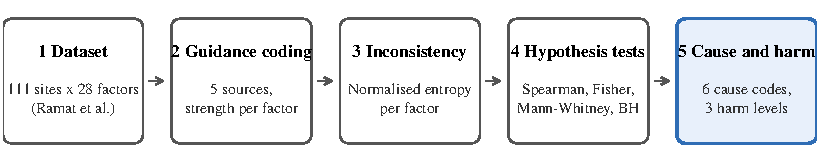
\includegraphics[width=\textwidth]{fig1.pdf}\caption{Methodology overview.}\label{fig:1}\end{figure*}

\subsection{Dataset}

We used the 111 × 28 score matrix published with the original study {[}2{]}, in which each website-factor pair is coded 0 (not applicable), 1 (non-match), 2 (partial match) or 3 (match), together with each website's global popularity rank, sector and cluster. In the first phase of this project we reproduced every factor rate in the original Table 2, the mean pairwise distance (0.57) and the three clusters exactly. As in the original study, a factor's implementation rate is the share of applicable websites coded as a partial or full match.

\subsection{Guidance Source Selection and Coding}

We selected five sources that implementers are most likely to consult: the FIDO Alliance Design Guidelines {[}3{]}, the W3C WebAuthn Level 3 Recommendation {[}4{]}, Google's passkey UX and developer guidance {[}5, 6{]}, Apple's passkey developer guidance {[}7{]} and Microsoft's passkey design guidelines {[}8{]}. All were read on 22 November 2026. We used the current FIDO text (latest patterns dated May 2024) rather than the June 2023 snapshot used by Ramat et al., because recommendations must target the text implementers read today.

For each factor we coded the strongest relevant statement in each source on a five-level scale: prescribed (MUST or a hard technical requirement) = 3, recommended (SHOULD, ``recommend'', or an element of a FIDO required pattern) = 2, optional (``consider'', ``can'', or a FIDO optional or security-key pattern) = 1, ambiguous or conflicting = 0.5, and discouraged or silent = 0. \emph{FIDO strength} is the FIDO score alone; \emph{guidance consensus} is a weighted mean of the five scores (range 0 to 3), with FIDO weighted at 70\% and WebAuthn, Google, Apple and Microsoft at 7.5\% each. We chose these weights because the FIDO guidelines are the reference text of this study; the unweighted sum is reported as a robustness check. Appendix A lists the codes and the decisive wording.

\subsection{Measuring Inconsistency}

Implementation rate and consistency measure different things. A factor implemented by 50\% of websites is maximally inconsistent, whereas one implemented by 3\% is highly consistent, albeit consistently absent. We therefore measured each factor's inconsistency as the normalised Shannon entropy of its three outcomes over applicable websites:

\begin{equation}
H_f = -\frac{1}{\log 3} \sum_{k \in \{1,2,3\}} p_{f,k} \log p_{f,k}
\end{equation}

where p(f,k) is the share of applicable websites with outcome k on factor f.~H = 0 means every website behaves the same, and H = 1 means an even split across the three outcomes.

\subsection{Hypothesis Testing}

We tested the relationship between guidance and consistency with Spearman's rank correlation across the 28 factors. We checked its robustness by removing duplicate factors, browser-default factors and factors applicable to fewer than 60 websites; by leaving out each guidance source in turn; with a 5,000-sample bootstrap and a 10,000-permutation test; and with a rank regression that controls for whether the browser supplies a behaviour by default.

At the website level we tested candidate causes derived from an earlier hypothesis-generation phase. Shared causes were tested through factor co-occurrence (Fisher's exact test and the φ coefficient), sector effects through Fisher's exact tests comparing a sector with all other websites, and site maturity through Mann-Whitney U tests on popularity rank. We applied Benjamini-Hochberg false discovery rate control {[}18{]} to the 23 confirmatory tests (Appendix B). We dated the browser features on which several factors depend from vendor documentation {[}9, 10{]}.

\subsection{Cause and Harm Classification}

Each factor that had not converged received one primary cause code and up to two secondary codes (Table 1), assigned from the convergent evidence above: guidance codes, co-occurrence, sector and rank effects, and browser timelines. We considered a factor converged if at least 90\% of applicable websites implement it and its entropy is at most 0.3.

\begin{table}[t]\centering\footnotesize\setlength{\tabcolsep}{3pt}\caption{Cause codes used to classify inconsistencies}\label{tab:1}
\begin{tabularx}{\columnwidth}{l>{\raggedright\arraybackslash}X>{\raggedright\arraybackslash}X}\toprule
\textbf{Code} & \textbf{Cause} & \textbf{Who can address it} \\ \midrule
G & Guideline missing, ambiguous, optional, outdated, or in conflict with another source & FIDO UX working group, platform vendors \\
P & Platform, browser or credential-manager behaviour & OS and browser vendors, W3C \\
T & Technical constraint or library default & Library and identity-provider vendors \\
L & Legacy architecture, such as password-first stacks or older 2FA schemas & The website \\
B & Deliberate business or risk decision & The website (often legitimate) \\
M & Measurement artefact of the original rubric & Researchers \\
\bottomrule\end{tabularx}\end{table}

We rated harm separately for usability and security on three levels. High means a user can lose access or an attacker can gain persistent access. Medium means a user is misled, cannot perform an expected action, or loses a signal that would reveal an attack. Low means a cosmetic or discoverability difference. Factors whose variation reflects a defensible business decision with low harm are reported as legitimate variance.

\subsection{Limitations}

This study has several limitations. By design we did not visit websites, log WebAuthn requests, or interview developers. Explanations that concern the options a website sends, such as the registration restriction discussed in Section 4.3, can therefore be supported or contradicted by the data but not directly confirmed.

One researcher coded the guidance and rated harm, and another author reviewed and accepted the codes; we did not compute inter-rater agreement. Leave-one-source-out analyses reduce, but do not eliminate, the influence of individual coding decisions. The source weights in the consensus score (FIDO 70\%, the other four sources 7.5\% each) were chosen by the authors; weighting all sources equally gives the same result (ρ = −0.46, p = 0.013). The guidance analysis rests on 28 data points, and the ordinal guidance scores are treated as interval values. The bootstrap interval for our main correlation is correspondingly wide.

We inherit the limitations of the original dataset: one platform (Windows 11 and Chrome), one evaluation period (February 2025 to February 2026), and a sample that over-represents large, English-language services. Website behaviour may have changed since. Because we compare websites against today's FIDO text, some gaps may appear larger than they were when a website was built. False discovery control covers only the 23 confirmatory tests; associations from the exploratory screen that we did not re-test should be read as hypotheses. Finally, all cause codes are best-supported explanations drawn from correlational evidence, not established causal effects.

\subsection{Ethics Statement}

This study analysed publicly released, website-level data and publicly available documents. It involved no human participants, no personal data, and no interaction with the websites studied, so it did not require ethics board review. We do not identify vulnerabilities in individual websites beyond what the original study published, and our findings concern aggregate design patterns.

\section{Results}

We first describe how current guidance covers the 28 factors (Section 4.1) and how guidance relates to consistency (Section 4.2). We then re-examine the Selective cluster (Section 4.3), report site-level drivers (Section 4.4), classify the causes of inconsistency by journey stage (Section 4.5), quantify lifecycle security exposure (Section 4.6), and assess which guideline problems contribute to inconsistency (Section 4.7).

\subsection{Guidance Coverage}

Guidance is sparse and rarely normative (Table 2). The FIDO guidelines contain no MUST or SHOULD; the only imperative is ``Require that people name the security key'', in a 2022 security-key pattern. Only two factors are backed by a normative SHOULD in any source (F12 Multicreation and F19 Fallback-Authentication, both in WebAuthn Level 3). Re-authentication before adding a passkey (F13) is addressed by a single Google page, and re-authentication before deleting one (F26) is addressed by no source.

We found seven direct conflicts between sources. Four affect measured factors. FIDO asks for passkeys \emph{above} passwords while Google presents them \emph{alongside} passwords (F02). FIDO now advises against a dedicated passkey sign-in button, which the original rubric scores as a required pattern (F17). FIDO offers a ``Use a security key'' option at creation, while Google's passkey checklist recommends \texttt{authenticatorAttachment:\ "platform"} for promoted creation (F09, F10). FIDO classifies passkey sign-up as optional, while Apple advises giving users ``a passkey from the start'' (F06). Three FIDO patterns are also outdated relative to WebAuthn Level 3: there is no automatic-upgrade pattern, the removal pattern anticipates a future ``Report API'' rather than the Signal API, and the security-key patterns frame keys as a second factor after a password.

\begin{table*}[t]\centering\scriptsize\setlength{\tabcolsep}{3pt}\caption{Guidance strength per factor and source. M = prescribed, S = recommended, O = optional, A = ambiguous or conflicting, X = discouraged, -- = silent. Rate from Ramat et al.~{[}1{]}; H = normalised entropy (Section 3.3).}\label{tab:2}
\begin{tabularx}{\textwidth}{>{\raggedright\arraybackslash}Xllccccccc}\toprule
\textbf{Factor} & \textbf{Stage} & \textbf{Rate} & \textbf{H} & \textbf{FIDO} & \textbf{WebAuthn} & \textbf{Google} & \textbf{Apple} & \textbf{Microsoft} & \textbf{Consensus (weighted)} \\ \midrule
F01 Promotion & Discovery & 90\% & 0.29 & S & -- & S & O & S & 1.78 \\
F02 Priority & Discovery & 36\% & 0.59 & S & -- & A & -- & -- & 1.44 \\
F03 HSK-Awareness & Discovery & 43\% & 0.62 & O & O & -- & -- & -- & 0.77 \\
F04 Educational-Resources & Discovery & 51\% & 0.77 & S & -- & S & -- & S & 1.70 \\
F05 Naming-Conventions & Discovery & 93\% & 0.24 & O & A & S & -- & O & 0.96 \\
F06 Registration-Setup & Setup & 25\% & 0.66 & O & -- & S & S & O & 1.08 \\
F07 OTP-Setup & Setup & 7\% & 0.24 & O & O & S & O & -- & 1.00 \\
F08 Settings-Setup & Setup & 97\% & 0.11 & S & -- & S & -- & S & 1.70 \\
F09 HSK-Setup & Setup & 82\% & 0.43 & O & O & A & -- & -- & 0.81 \\
F10 Cross-Device-Setup & Setup & 82\% & 0.43 & O & O & O & -- & -- & 0.85 \\
F11 Recovery-Setup & Setup & 3\% & 0.14 & O & -- & S & O & -- & 0.92 \\
F12 Multicreation & Setup & 95\% & 0.19 & O & S & S & A & -- & 1.04 \\
F13 Setup-Authentication & Setup & 30\% & 0.65 & -- & -- & S & -- & -- & 0.15 \\
F14 Setup-Notification & Setup & 80\% & 0.45 & O & -- & S & -- & -- & 0.85 \\
F15 Update-Option & Setup & 47\% & 0.63 & A & -- & A & -- & -- & 0.39 \\
F16 Update-Notification & Setup & 53\% & 0.63 & O & -- & -- & -- & -- & 0.70 \\
F17 Sign-In-UI & Usage & 84\% & 0.40 & X & -- & X & -- & A & 0.04 \\
F18 Autofill-Feature & Usage & 42\% & 0.62 & S & O & S & O & S & 1.85 \\
F19 Fallback-Authentication & Usage & 98\% & 0.08 & S & S & S & S & S & 2.00 \\
F20 Cross-Device-Usage & Usage & 96\% & 0.53 & O & O & -- & -- & -- & 0.77 \\
F21 HSK-Usage & Usage & 96\% & 0.54 & O & O & -- & -- & -- & 0.77 \\
F22 Mobile-App-Usage & Usage & 63\% & 0.60 & O & O & -- & M & -- & 1.00 \\
F23 Management-UI & Usage & 93\% & 0.24 & S & O & S & -- & S & 1.78 \\
F24 Delete-Option & Deletion & 97\% & 0.11 & S & O & S & -- & S & 1.78 \\
F25 Authenticator-Cleanup & Deletion & 23\% & 0.49 & O & O & S & -- & -- & 0.92 \\
F26 Deletion-Authentication & Deletion & 30\% & 0.67 & -- & -- & -- & -- & -- & 0.00 \\
F27 Deletion-Notification & Deletion & 69\% & 0.57 & O & -- & -- & -- & -- & 0.70 \\
F28 Deletion-Confirmation & Deletion & 91\% & 0.61 & O & -- & A & -- & -- & 0.74 \\
\bottomrule\end{tabularx}\end{table*}

\subsection{Guidance Agreement and Consistency}

Factors on which guidance sources agree are implemented more uniformly (Spearman ρ = −0.45, p = 0.016; permutation p = 0.017; bootstrap 95\% CI −0.79 to −0.04), as shown in Figure 2. FIDO strength alone is a weaker predictor (ρ = −0.36, p = 0.058): it is the agreement of several sources, not FIDO's text by itself, that carries the effect.

\begin{figure}[t]\centering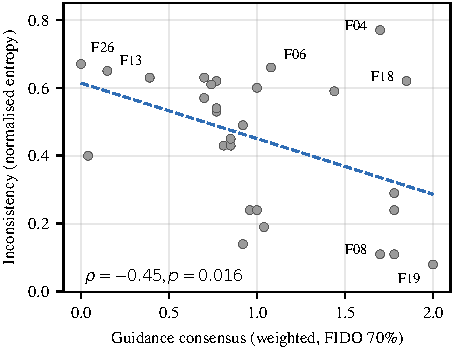
\includegraphics[width=\columnwidth]{fig2.pdf}\caption{Guidance consensus and inconsistency across the 28 factors. Dashed line: least-squares trend.}\label{fig:2}\end{figure}

The relationship holds across all robustness checks (Table 3). An obvious confound is that some behaviours, such as fallback sign-in, cross-device sign-in and deletion, are supplied by the browser or by libraries by default. In a rank regression that includes a browser-default indicator, consensus remains significant (β = −0.38, p = 0.033) alongside the default indicator (β = −0.50, p = 0.042). Both contribute, and neither explains the other away.

\begin{table}[t]\centering\footnotesize\setlength{\tabcolsep}{3pt}\caption{Robustness of the consensus--inconsistency correlation}\label{tab:3}
\begin{tabularx}{\columnwidth}{Xccc}\toprule
\textbf{Check} & \textbf{Factors} & \textbf{ρ} & \textbf{p} \\ \midrule
All factors (FIDO 70\%, others 7.5\% each) & 28 & −0.45 & 0.016 \\
Without exact duplicates F10, F21 & 26 & −0.45 & 0.021 \\
Without browser-default F20, F21 & 26 & −0.45 & 0.021 \\
Without small-n factors F07, F11, F16 & 25 & −0.43 & 0.031 \\
Without Google (largest decrease) & 28 & −0.42 & 0.027 \\
Without Apple (largest increase) & 28 & −0.51 & 0.005 \\
Equal weights (unweighted sum) & 28 & −0.46 & 0.013 \\
FIDO and WebAuthn 35\% each, others 10\% each & 28 & −0.48 & 0.010 \\
FIDO alone & 28 & −0.36 & 0.058 \\
\bottomrule\end{tabularx}\end{table}

The outliers show where guidance is not the driver. F02 Priority (36\%) and F18 Autofill-Feature (42\%) are recommended yet unevenly implemented. F17 Sign-In-UI is discouraged by FIDO yet implemented by 84\%, because websites treat a passkey button and autofill as substitutes: 16 of the 18 websites without a button offer autofill (φ = −0.41, q \textless{} 0.001).

\subsection{Re-analysis of the Selective Cluster}

Ramat et al.~grouped 20 of the 111 websites (18\%) into a ``Selective Implementers'' cluster. Examples include PayPal, Target, Best Buy, Binance, Cash App and Nintendo. On these websites, users cannot create a passkey on a hardware security key or on a phone through the cross-device flow: within the cluster, F09 and F10 are implemented by 0\% of websites. Yet 16 of the 20 still accept a security key or a phone at sign-in, which the original study scored as partial matches on F20 and F21. In plain terms, these websites let users sign in with authenticators that they do not let users register.

F09 HSK-Setup and F10 Cross-Device-Setup fail on exactly the same 20 websites (φ = 1.0, q \textless{} 0.001), which form the entire Selective cluster. F20 Cross-Device-Usage and F21 HSK-Usage are also identical (φ = 1.0), and their partial matches are defined by the same F09/F10 failure. A single registration-time cause is therefore counted four times in the distance metric. Removing only the duplicates F10 and F21 moves 16 of the 20 Selective websites into the Standard cluster (Appendix D).

The pattern, in which users cannot register a security key or phone but can sign in with either, matches a registration request restricted to the device's own authenticator. This is the effect of \texttt{authenticatorAttachment:\ "platform"}, which Google's checklist recommends for promoted passkey creation and which FIDO's security-key patterns oppose. The cluster is concentrated by sector: 12 of its 20 websites are e-commerce or finance services, so 43\% of those two sectors are Selective against 6\% of IT websites (odds ratio 12.0, q \textless{} 0.001). We conclude that the cluster most likely reflects a technical setting chosen for risk reasons and endorsed by one guidance source. Because we did not observe registration requests, this explanation is supported but not confirmed.

\subsection{Site Attributes}

After false discovery control, 21 of the 23 confirmatory tests remain significant (Appendix B). Three patterns explain causes. First, finance websites follow a risk-averse profile: they rarely offer passkeys at account creation (F06: 1 of 14), re-authenticate before adding a passkey more often (F13: 57\% vs 26\%, q = 0.034), mention security keys more often (F03: 71\% vs 39\%, q = 0.046) and restrict security-key registration more often (F09: 57\% vs 86\%, q = 0.029). Second, mature websites notify and educate: websites that send a notification when a passkey is added are far more popular (median rank 13,139 vs 936,085, q = 0.001), as are websites with educational content (q = 0.032). Third, passkey sign-up is a newcomer's feature: websites offering it are less popular (median rank 771,768 vs 14,088, q = 0.021), and 5 of the 6 authentication-provider websites offer it against 22\% of others (q = 0.010). The association between popularity and autofill (p = 0.048) does not survive correction.

\subsection{Root Causes by Journey Stage}

For the 21 factors that have not converged, the most likely primary cause is a guideline problem for 8, a technical constraint or default for 4, legacy architecture for 4, a deliberate business decision for 3, and a measurement artefact for 2 (Table 4). Seven factors have converged: F01, F05, F08, F12, F19, F23 and F24. Figure 3 places each non-converged factor by inconsistency and harm.

\subsubsection{Discovery}

Discovery differences are mostly low in harm. Priority (F02) is inconsistent because FIDO and Google disagree and because older settings pages place passkeys inside an existing two-factor section. Security-key awareness (F03) follows audience: regulated finance mentions keys most, while FIDO's 2022 security-key pattern still frames keys as a second factor. Educational content (F04) follows help-centre maturity rather than guidance, since three sources recommend it yet it remains the most inconsistent factor in the dataset (H = 0.77).

\subsubsection{Setup}

Setup holds two of the five high-harm factors. The F09/F10 registration restriction (Section 4.3) is a technical setting with a business motive and a guidance conflict behind it, and leaves users with authenticators that sign-in accepts but registration refuses. Re-authentication before adding a passkey (F13) is unguided and set by site-wide step-up policy. The low rate for passkey creation after OTP sign-in (F07) reflects FIDO's missing automatic-upgrade pattern, late browser support, and a small applicable base (27 websites). Passkey sign-up (F06) and passkey creation during recovery (F11) are deliberate risk decisions that we treat as legitimate variance. Notifications (F14, F16) follow the maturity of a website's security-email pipeline.

\subsubsection{Usage}

Web-to-app passkey use (F22) fails on 23 of 62 applicable websites. Its cause is technical: associated-domain files and the choice of RP identifier, often owned by separate web and app teams. Autofill (F18) is strongly recommended yet implemented by only 42\%, consistent with identifier-first and hosted login pages that predate conditional mediation. The apparent inconsistency in cross-device and security-key sign-in (F20, F21) is a measurement artefact inherited from F09 and F10.

\subsubsection{Deletion}

Deletion contains the second unguided security gap, re-authentication before deleting a passkey (F26). Authenticator cleanup (F25) is low because FIDO's removal pattern predates the Signal API, and a website that calls the Signal API is still scored as a non-match. Deletion confirmation (F28) appears converged at 91\%, but 83 of 96 applicable websites are only partial matches: nearly all show a confirmation dialog, and almost none warns before the last passkey is removed.

\begin{table*}[t]\centering\scriptsize\setlength{\tabcolsep}{3pt}\caption{Primary cause and harm for the 21 non-converged factors, ordered by harm}\label{tab:4}
\begin{tabularx}{\textwidth}{>{\raggedright\arraybackslash}p{3.3cm}cc>{\raggedright\arraybackslash}X>{\raggedright\arraybackslash}p{1.1cm}ll>{\raggedright\arraybackslash}X}\toprule
\textbf{Factor} & \textbf{Rate} & \textbf{H} & \textbf{Primary cause} & \textbf{Secondary} & \textbf{Usability harm} & \textbf{Security harm} & \textbf{Key evidence} \\ \midrule
F13 Setup-Authentication & 30\% & 0.65 & G: silent in 4 of 5 sources & B, L & Low & \textbf{High} & φ = 0.73 with F26; 0 of 6 auth providers \\
F26 Deletion-Authentication & 30\% & 0.67 & G: silent in all sources & B, L & Low & \textbf{High} & 70 of 108 websites do neither \\
F09 HSK-Setup & 82\% & 0.43 & T: platform-only registration & B, G & \textbf{High} & Low & φ = 1.0 with F10; sector OR = 12 \\
F10 Cross-Device-Setup & 82\% & 0.43 & T: same as F09 & B, G & \textbf{High} & Low & Identical to F09 \\
F22 Mobile-App-Usage & 63\% & 0.60 & T: associated domains, RP ID & L & \textbf{High} & Low & 23 of 62 fail \\
F25 Authenticator-Cleanup & 23\% & 0.49 & G: predates Signal API & P, M & Medium & Low & Signal API in Chrome 132 \\
F07 OTP-Setup & 7\% & 0.24 & G: no automatic-upgrade pattern & P, M & Medium & Low & 27 applicable websites \\
F28 Deletion-Confirmation & 91\% & 0.61 & G: last-passkey case unspecified & M & Medium & Low & 83 of 96 partial \\
F18 Autofill-Feature & 42\% & 0.62 & L: identifier-first login & T, P & Medium & Low & Recommended by 3 sources \\
F04 Educational-Resources & 51\% & 0.77 & B: help-centre maturity & G & Medium & Low & Rank q = 0.032 \\
F14 Setup-Notification & 80\% & 0.45 & L: security-email pipeline & G & Low & Medium & Rank q = 0.001 \\
F27 Deletion-Notification & 69\% & 0.57 & L: same pipeline & M & Low & Medium & φ = 0.40 with F14 \\
F11 Recovery-Setup & 3\% & 0.14 & B: recovery risk & G, L & Low & Medium & No proofing level in any source \\
F02 Priority & 36\% & 0.59 & G: FIDO vs Google & L & Low & Low & Recommended yet 36\% \\
F03 HSK-Awareness & 43\% & 0.62 & G: optional, 2FA-era & B & Low & Low & Finance 71\% \\
F17 Sign-In-UI & 84\% & 0.40 & G: discouraged vs rubric & M & Low & Low & 16 of 18 non-matches use autofill \\
F16 Update-Notification & 53\% & 0.63 & L & B & Low & Low & Low-risk event \\
F06 Registration-Setup & 25\% & 0.66 & B: recovery risk & L & Low & Low & Finance 1 of 14 \\
F15 Update-Option & 47\% & 0.63 & T: automatic naming & B & Low & Low & Legitimate variance \\
F20 Cross-Device-Usage & 96\% & 0.53 & M: partial defined by F10 & P & Low & Low & Browser default \\
F21 HSK-Usage & 96\% & 0.54 & M: partial defined by F09 & P & Low & Low & Browser default \\
\bottomrule\end{tabularx}\end{table*}

\begin{figure}[t]\centering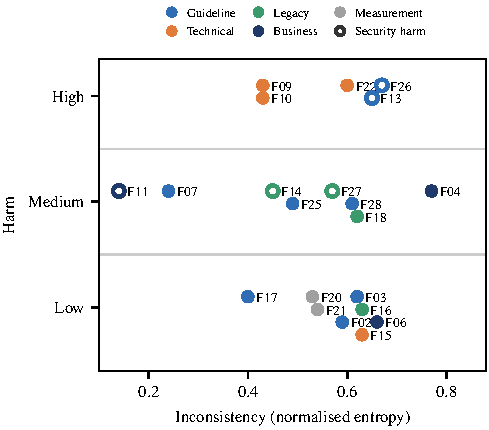
\includegraphics[width=\columnwidth]{fig3.pdf}\caption{Inconsistency and harm of the 21 non-converged factors, coloured by primary cause. Rings mark security harm.}\label{fig:3}\end{figure}

\subsection{Lifecycle Security Exposure}

Of the 108 websites where both factors apply, 70 (65\%) re-authenticate users neither when a passkey is added nor when one is deleted, and only 26 do both. Re-authentication is all-or-nothing per website (F13 and F26 agree on 96 of 108 websites, φ = 0.73), which indicates a site-wide step-up policy rather than a passkey-specific decision. Even the six authentication-provider websites, whose business is passkeys, re-authenticate for neither action. On 12 websites there is no re-authentication and no notification for either action. On these websites, anyone with brief session access could register their own passkey for persistent access or delete the owner's passkeys without the owner being informed, the persistence and lock-out risk raised by Ramat et al.~{[}1{]} and Daffalla et al.~{[}13{]}.

\subsection{Guideline Problems and Their Contribution}

We counted a guideline problem as contributing to inconsistency only when the data show a matching inconsistency and no stronger cause explains it better (Table 5). Of the twelve problems we identified, the missing lifecycle guidance and the attachment conflict contribute most clearly. Two apparent gaps are not attributable to the guidelines: web-to-app use (F22) is well covered by platform documentation, and passkey sign-up (F06) is avoided for recovery-risk reasons that stronger text would not change.

\begin{table*}[t]\centering\scriptsize\setlength{\tabcolsep}{3pt}\caption{Problems in the FIDO guidelines and whether they contribute to inconsistency}\label{tab:5}
\begin{tabularx}{\textwidth}{>{\raggedright\arraybackslash}X>{\raggedright\arraybackslash}p{1.4cm}>{\raggedright\arraybackslash}p{1.6cm}>{\raggedright\arraybackslash}p{2cm}>{\raggedright\arraybackslash}X}\toprule
\textbf{Problem} & \textbf{Type} & \textbf{Factors} & \textbf{Contributes?} & \textbf{Evidence} \\ \midrule
No MUST/SHOULD language; patterns can be combined ``to match your unique business needs'' & Structural & All & Yes, moderately & FIDO alone ρ = −0.36; F02, F18 low despite recommendation \\
No versioning or changelog & Structural & All & Indirectly & Original June 2023 text cannot be reproduced \\
Notification guidance in a separate communications page & Structural & F14, F16, F27 & Weakly & Notification follows site maturity \\
Re-authentication for adding or deleting not mentioned & Missing & F13, F26 & Yes, strongly & 65\% do neither; 0 of 6 auth providers \\
No identity-proofing level for recovery & Missing & F11 & Partly & Risk policy is the stronger cause \\
Card contents and last-passkey behaviour unspecified & Missing & F23, F28 & Yes, for F28 & 83 of 96 partial \\
No automatic-upgrade pattern & Outdated & F01, F06, F07 & Yes, with timing & Supported by Safari 18 and Chrome 136 \\
Removal pattern predates the Signal API & Outdated & F25 & Yes, with measurement & 23\%; Signal API available \\
Security-key patterns framed as 2FA & Outdated & F03, F09, F21 & Partly & Sector explains more \\
``Above'' vs ``alongside'' passwords & Conflict & F02 & Yes & Recommended yet 36\% \\
Security-key option vs platform-only advice & Conflict & F09, F10 & Yes & Selective cluster \\
Dedicated button discouraged, autofill unavailable on some clients & Ambiguous & F17, F18 & Yes & φ = −0.41 \\
\bottomrule\end{tabularx}\end{table*}

Browser timing also matters. The Signal API shipped in Chrome 132 {[}10{]}, and conditional create shipped in Chrome 136 on desktop in spring 2025 {[}9{]}, at or near the start of the evaluation period. Appendix C lists the dates.

\section{Discussion}

\subsection{Why Passkey Implementations Diverge}

Our findings show that passkey inconsistency has several causes, and that guidelines are one of them rather than the main one. Agreement among guidance sources explains a moderate share of the variation across factors. Within factors, sector risk policy, website maturity and browser defaults explain more. The most valuable change to the guidelines is therefore not more patterns. It is clearer force on a small number of safety-relevant patterns, because that is where weak guidance and real harm coincide.

Not all inconsistency is undesirable. Finance websites that refuse passkey-only accounts, or that refuse to issue a passkey through a recovery flow, are making a defensible security trade-off, and a guideline that forced uniformity would lower security. Our harm classification separates these cases so that recommendations target only harmful variance. We do not recommend standardising passkey sign-up (F06), passkey creation during recovery (F11) or passkey renaming (F15).

\subsection{Recommendations for the FIDO Alliance Design Guidelines}

Table 6 lists ten recommendations for the FIDO Alliance. Priority 1 marks a high-harm factor with a guideline cause, priority 2 a medium-harm factor or a measured conflict, and priority 3 clarity and maintenance. The most important is a lifecycle-security pattern (R1), because it addresses the only high-harm gap that no guidance source covers.

\begin{table*}[t]\centering\footnotesize\setlength{\tabcolsep}{3pt}\caption{Recommendations for the FIDO Alliance}\label{tab:6}
\begin{tabularx}{\textwidth}{lc>{\raggedright\arraybackslash}X>{\raggedright\arraybackslash}p{2.2cm}>{\raggedright\arraybackslash}p{3.4cm}}\toprule
\textbf{\#} & \textbf{Priority} & \textbf{Recommendation} & \textbf{Factors} & \textbf{Evidence} \\ \midrule
R1 & 1 & Add a lifecycle-security pattern: require recent user verification before adding or deleting a passkey, with a short grace period after sign-in, and an out-of-band notification for both actions & F13, F26, F14, F27 & 65\% do neither; 0 of 6 auth providers \\
R2 & 1 & Adopt normative strength labels (MUST, SHOULD, MAY) per pattern element, and separate safety-relevant elements from brand choices & All & Consensus ρ = −0.45 vs FIDO alone −0.36 \\
R3 & 1 & Resolve the attachment conflict: registration should not restrict \texttt{authenticatorAttachment} without a documented reason, and a restricted promoted prompt must be paired with an unrestricted option in settings & F09, F10, F20, F21 & Selective cluster; sector OR = 12 \\
R4 & 2 & Add an automatic-upgrade pattern (conditional create after password or OTP sign-in), including the capability check WebAuthn Level 3 asks for & F01, F06, F07 & Safari 18, Chrome 136; FIDO silent \\
R5 & 2 & Update the removal pattern to use the Signal API, with the manual credential-manager message as a fallback & F25 & 23\%; Signal API since Chrome 132 \\
R6 & 2 & Specify the last-passkey case: warn and name the remaining fallback; block deletion only when no other sign-in method remains & F28 & 83 of 96 partial \\
R7 & 2 & Agree one priority rule with platform vendors for passkeys relative to passwords and 2FA & F02 & 36\%; FIDO vs Google conflict \\
R8 & 2 & Clarify button versus autofill: autofill as the primary path, a button as a fallback for clients without conditional mediation & F17, F18 & φ = −0.41 \\
R9 & 3 & Publish versioned guidelines with a changelog and dated snapshots & All & No version numbers since 2022 \\
R10 & 3 & Merge notification templates into their patterns and rewrite security-key patterns as passkey patterns & F03, F14, F16, F27 & Split text; 2022 framing \\
\bottomrule\end{tabularx}\end{table*}

\subsection{Recommendations for Websites and Platforms}

Website developers can address most harmful inconsistencies without waiting for revised guidance (Table 7). Platform, browser and library vendors control the defaults that drive much of the convergence we observed, so changes there would propagate to many websites at once (Table 8).

\begin{table*}[t]\centering\footnotesize\setlength{\tabcolsep}{3pt}\caption{Recommended practices for website developers}\label{tab:7}
\begin{tabularx}{\textwidth}{l>{\raggedright\arraybackslash}X>{\raggedright\arraybackslash}p{1.6cm}>{\raggedright\arraybackslash}p{4cm}}\toprule
\textbf{\#} & \textbf{Practice} & \textbf{Factors} & \textbf{Rationale} \\ \midrule
W1 & Require fresh user verification before adding or removing a passkey, reusing the existing step-up policy & F13, F26 & Prevents session-hijack persistence and lock-out \\
W2 & Notify the account owner of every passkey addition and deletion, with a ``this wasn't me'' path & F14, F27 & Detection when W1 fails \\
W3 & If a promoted prompt uses \texttt{authenticatorAttachment:\ "platform"}, keep an unrestricted option in settings & F09, F10 & Registration should accept what sign-in accepts \\
W4 & Add \texttt{autocomplete="webauthn"} and conditional mediation to the first identifier field, including identifier-first and hosted pages & F18 & Recommended by three sources; 42\% today \\
W5 & Call the Signal API after deletion and on unknown-credential errors, with a manual message as fallback & F25 & Removes orphaned credentials \\
W6 & Publish associated-domain files and use one RP ID across web and app & F22 & 23 of 62 fail web-to-app use \\
W7 & Warn before the last passkey is deleted and name the remaining method & F28 & Prevents unexpected lock-out \\
W8 & Use automatic upgrades after password sign-in instead of additional banners & F01, F07 & Fewer prompts, more passkeys \\
W9 & Name passkeys automatically from the authenticator's AAGUID; offer renaming as a secondary action & F15 & Legitimate variance \\
\bottomrule\end{tabularx}\end{table*}

\begin{table*}[t]\centering\footnotesize\setlength{\tabcolsep}{3pt}\caption{Requests to platform, browser and library vendors}\label{tab:8}
\begin{tabularx}{\textwidth}{l>{\raggedright\arraybackslash}X>{\raggedright\arraybackslash}p{2.6cm}>{\raggedright\arraybackslash}p{3.6cm}}\toprule
\textbf{\#} & \textbf{Request} & \textbf{Factors} & \textbf{Rationale} \\ \midrule
P1 & Library and identity-provider defaults should not restrict attachment, and should ship autofill, notification hooks and a re-authentication gate for credential changes & F09, F10, F13, F18, F26 & Defaults predict consistency (β = −0.50) \\
P2 & Implement the Signal API in Firefox and on all Safari platforms & F25 & Chrome-only for most of the evaluation period \\
P3 & Qualify Google's platform-only attachment recommendation in line with R3 & F09, F10 & Source conflict \\
P4 & Offer the same authenticator choices at registration and sign-in when the RP does not restrict them & F09, F10, F20, F21 & Mismatch confuses users \\
\bottomrule\end{tabularx}\end{table*}

\subsection{Implications for the Comparative Framework}

The original framework overstates some inconsistency. Four factors encode one registration cause, and three are scored against guidance that has since changed or was misattributed: F04 is labelled as having no FIDO source although the account-settings pattern contains it, F17 is scored as required although FIDO now discourages it, and F27 requires an email or push notification although its cited source is an in-app message. We recommend that replication studies merge F09 with F10 and F20 with F21, credit a Signal API call as a match for F25, split F28 into a confirmation dialog and a last-passkey warning, and report entropy alongside implementation rate. With these changes, longitudinal comparisons would measure website behaviour rather than rubric structure.

\subsection{Future Work}

Three studies would turn our supported explanations into confirmed ones. First, logging the registration options sent by the 20 Selective websites and a set of Standard controls would directly test the platform-only explanation in Section 4.3. Second, a developer survey could establish why re-authentication for passkey changes is so rarely implemented, and whether a FIDO pattern would change that decision. Third, a user study could measure how much confusion arises when registration and sign-in support different authenticators, and whether lifecycle notifications help users detect unauthorised passkey changes. Repeating our analysis on the next version of the FIDO guidelines would also show whether stronger guidance increases consistency over time.

\section{Conclusion}

Passkeys promise a consistent, phishing-resistant sign-in experience, but their implementations diverge across websites. In this study, we explained why, using the per-site data of a 111-website, 28-factor evaluation and a structured coding of five guidance sources. Where guidance sources agree, websites converge; where guidance is silent, non-normative, outdated or contradictory, they diverge. Much of the remaining variation reflects browser defaults, legacy login and notification systems, and deliberate risk decisions in finance and commerce, and part of it reflects the original rubric itself.

The differences that matter most are few. Passkey addition and deletion are unprotected by re-authentication on 65\% of websites, and some websites refuse to register the same authenticators they accept at sign-in. Both can be addressed with a small number of normative, versioned changes to the FIDO Alliance Design Guidelines and matching changes to library defaults, without restricting legitimate product decisions. We hope our cause-and-harm framework helps guideline authors, implementers and researchers focus on the inconsistencies that harm users.

\section*{Acknowledgments}

We thank our supervisor, Shweta Komari, for guidance and feedback throughout this project.

\section*{Availability}

Our analysis scripts, outputs, figures and the LaTeX source of this paper are available at \url{https://github.com/devsinghshekhawat11/passkeys-analysis}. The website-level dataset is the supplementary material of Ramat et al., available at \url{https://zenodo.org/records/20709272}.

\begin{thebibliography}{99}\small\raggedright
\bibitem{r1} Bernhardt Ramat, David Kartchner, Michael Clark, and Kent Seamons. Passkeys in the wild: A systematic study of FIDO2 user experience consistency across websites. In Twenty-Second Symposium on Usable Privacy and Security (SOUPS), August 2026. URL: https://www.usenix.org/conference/soups2026/presentation/ramat.
\bibitem{r2} Bernhardt Ramat et al.~Supplementary materials for ``Passkeys in the wild'', 2026. URL: https://zenodo.org/records/20709272.
\bibitem{r3} FIDO Alliance. Design guidelines. Passkey Central, pattern pages dated May 2022 to May 2024. Accessed 2026-11-22. URL: https://www.passkeycentral.org/design-guidelines/.
\bibitem{r4} W3C. Web Authentication: An API for accessing public key credentials, Level 3. W3C Recommendation, 2026. URL: https://www.w3.org/TR/webauthn-3/.
\bibitem{r5} Google LLC. Passkeys user interface design. Google Developers documentation; last updated 16 September 2025. URL: https://developers.google.com/identity/passkeys/ux/user-interface-design.
\bibitem{r6} Google LLC. Passkeys developer guide, user journeys, and passkey checklist, 2025. URL: https://developers.google.com/identity/passkeys.
\bibitem{r7} Apple Inc.~Passkeys. Developer overview and WWDC24 session 10125, 2024. URL: https://developer.apple.com/passkeys/.
\bibitem{r8} Microsoft Corporation. Design guidelines for passkeys. Microsoft Learn documentation; last updated 9 September 2024. URL: https://learn.microsoft.com/en-us/windows/apps/develop/security/design.
\bibitem{r9} Google LLC. Automatically create passkeys in Google Password Manager on Chrome desktop. Chrome for Developers, 9 May 2025. URL: https://developer.chrome.com/blog/passkey-automatic-upgrades.
\bibitem{r10} Google LLC. Keep passkeys consistent with credentials on your server with the Signal API. Chrome for Developers, November 2024. URL: https://developer.chrome.com/docs/identity/webauthn-signal-api.
\bibitem{r11} Sanam Ghorbani Lyastani, Michael Backes, and Sven Bugiel. A systematic study of the consistency of two-factor authentication user journeys on top-ranked websites. In Network and Distributed System Security (NDSS) Symposium, March 2023.
\bibitem{r12} Leona Lassak, Elleen Pan, Blase Ur, and Maximilian Golla. Why aren't we using passkeys? Obstacles companies face deploying FIDO2 passwordless authentication. In 33rd USENIX Security Symposium, pages 7231--7248, August 2024.
\bibitem{r13} Alaa Daffalla, Arkaprabha Bhattacharya, Jacob Wilder, Rahul Chatterjee, Nicola Dell, Rosanna Bellini, and Thomas Ristenpart. A framework for abusability analysis: The case of passkeys in interpersonal threat models. In 34th USENIX Security Symposium, pages 7819--7838, August 2025.
\bibitem{r14} Eva Gerlitz, Maximilian Häring, Charlotte Theresa Mädler, Matthew Smith, and Christian Tiefenau. Adventures in recovery land: Testing the account recovery of popular websites when the second factor is lost. In Nineteenth Symposium on Usable Privacy and Security (SOUPS), pages 227--243, August 2023.
\bibitem{r15} Sabrina Klivan, Sandra Höltervennhoff, Nicolas Huaman, Alexander Krause, Lucy Simko, Yasemin Acar, and Sascha Fahl. ``We've disabled MFA for you'': An evaluation of the security and usability of multi-factor authentication recovery deployments. In ACM CCS, pages 3138--3152, 2023.
\bibitem{r16} Sanam Ghorbani Lyastani, Michael Schilling, Michaela Neumayr, Michael Backes, and Sven Bugiel. Is FIDO2 the kingslayer of user authentication? A comparative usability study of FIDO2 passwordless authentication. In IEEE Symposium on Security and Privacy, pages 268--285, 2020.
\bibitem{r17} Nicolas Huaman, Sabrina Klivan, Marten Oltrogge, Yasemin Acar, and Sascha Fahl. They would do better if they worked together: The case of interaction problems between password managers and websites. In IEEE Symposium on Security and Privacy, pages 1367--1381, 2021.
\bibitem{r18} Yoav Benjamini and Yosef Hochberg. Controlling the false discovery rate: A practical and powerful approach to multiple testing. Journal of the Royal Statistical Society: Series B, 57(1):289--300, 1995.
\bibitem{r19} Nielsen Norman Group. Maintain consistency and adhere to standards, January 2021. URL: https://www.nngroup.com/articles/consistency-and-standards/.
\end{thebibliography}

\appendix

\section{Guidance Codebook}

Each source was coded at the strength of its strongest statement relevant to the factor, using the scale in Section 3.2. When two statements in the same source disagreed, the source was coded A. Statements about the authenticator's own user verification were not counted as RP re-authentication (F13, F26). The decisive wording for the factors discussed in the paper is summarised below; the full extraction is available with our supplementary materials.

\begin{itemize}
\tightlist
\item
  \textbf{F02 Priority.} FIDO: ``place the passkeys UI above passwords''. Google: present passkeys ``alongside passwords and other methods''.
\item
  \textbf{F04 Educational-Resources.} FIDO account-settings pattern includes ``What are passkeys?'' messaging and a ``Learn more'' link; Google: make passkey information ``visible in the user interface by default''.
\item
  \textbf{F07 OTP-Setup.} FIDO: introduce passkeys ``immediately after they complete an SMS OTP authentication''. Google checklist: ``Automatically create a passkey (conditional create)''. No FIDO automatic-upgrade pattern.
\item
  \textbf{F09/F10 HSK- and Cross-Device-Setup.} FIDO management pattern: a ``Use a security key'' call to action. Google checklist: ``Specify `platform' as the authenticator attachment value'' for promoted creation.
\item
  \textbf{F12 Multicreation.} WebAuthn: ``Relying Parties SHOULD allow and encourage users to register multiple credentials''.
\item
  \textbf{F13 Setup-Authentication.} Google: ``Verify the user with the strongest authentication method available'' before creating a passkey. FIDO, WebAuthn, Apple, Microsoft: silent.
\item
  \textbf{F17 Sign-In-UI.} FIDO sign-in pattern on a dedicated passkey button: ``it is advised to avoid it''. Android guidance: do not display a separate button per sign-in method.
\item
  \textbf{F18 Autofill-Feature.} FIDO: ``Enable autofill by adding autocomplete=`webauthn' to the username input field''. WebAuthn: conditional mediation is optional.
\item
  \textbf{F19 Fallback-Authentication.} FIDO: ``Support graceful fallback to other sign-in methods''; WebAuthn SHOULD on additional authenticators or account recovery.
\item
  \textbf{F25 Authenticator-Cleanup.} FIDO: ``Inform people to remove the passkey from their credential manager'', anticipating a future ``Report API''. WebAuthn Level 3: RPs ``SHOULD prefer'' signalAllAcceptedCredentials when the user is signed in.
\item
  \textbf{F26 Deletion-Authentication.} Silent in all five sources.
\item
  \textbf{F28 Deletion-Confirmation.} FIDO: confirmation dialog and, for the last passkey, ``inform people of the fallback method''; silent on blocking deletion.
\end{itemize}

\section{Statistical Tests}

\begin{table}[t]\centering\footnotesize\setlength{\tabcolsep}{3pt}\caption{Confirmatory website-level tests with Benjamini-Hochberg correction (23 tests). Co-occurrence and sector tests use Fisher's exact test; rank tests use Mann-Whitney U.}\label{tab:9}
\begin{tabularx}{\columnwidth}{>{\raggedright\arraybackslash}Xlll}\toprule
\textbf{Test} & \textbf{p} & \textbf{q} & \textbf{Significant} \\ \midrule
F09 \textasciitilde{} F10 co-occurrence & 1.9e-22 & 4.3e-21 & Yes \\
F13 \textasciitilde{} F26 co-occurrence & 7.6e-14 & 8.7e-13 & Yes \\
F20 \textasciitilde{} F21 co-occurrence & 1.7e-07 & 1.3e-06 & Yes \\
F17 \textasciitilde{} F18 co-occurrence & 1.3e-05 & 7.8e-05 & Yes \\
F14 \textasciitilde{} F27 co-occurrence & 9.9e-05 & 0.00046 & Yes \\
Selective cluster: e-commerce and finance vs rest & 0.00026 & 0.00098 & Yes \\
F14 vs popularity rank & 0.00033 & 0.0011 & Yes \\
F04 \textasciitilde{} F03 co-occurrence & 0.00051 & 0.0015 & Yes \\
F06 authentication providers vs rest & 0.0038 & 0.0096 & Yes \\
F06 vs popularity rank & 0.0093 & 0.021 & Yes \\
F27 authentication providers vs rest & 0.011 & 0.024 & Yes \\
F25 vs popularity rank & 0.013 & 0.024 & Yes \\
F14 authentication providers vs rest & 0.014 & 0.024 & Yes \\
F16 \textasciitilde{} F27 co-occurrence & 0.015 & 0.025 & Yes \\
F09 finance vs rest & 0.019 & 0.029 & Yes \\
F04 vs popularity rank & 0.022 & 0.032 & Yes \\
F03 \textasciitilde{} F09 co-occurrence & 0.025 & 0.034 & Yes \\
F13 finance vs rest & 0.026 & 0.034 & Yes \\
F19 vs popularity rank & 0.032 & 0.039 & Yes \\
F03 finance vs rest & 0.040 & 0.046 & Yes \\
F22 finance vs rest & 0.042 & 0.046 & Yes \\
F18 vs popularity rank & 0.048 & 0.050 & No \\
F14 \textasciitilde{} F16 co-occurrence & 0.45 & 0.45 & No \\
\bottomrule\end{tabularx}\end{table}

\section{Browser Feature Timeline}

\begin{table*}[t]\centering\footnotesize\setlength{\tabcolsep}{3pt}\caption{Availability of WebAuthn features that several factors depend on, relative to the February 2025 to February 2026 evaluation period}\label{tab:10}
\begin{tabularx}{\textwidth}{>{\raggedright\arraybackslash}X>{\raggedright\arraybackslash}p{1.6cm}>{\raggedright\arraybackslash}p{2.8cm}>{\raggedright\arraybackslash}p{1.6cm}>{\raggedright\arraybackslash}p{1.8cm}>{\raggedright\arraybackslash}X}\toprule
\textbf{Feature} & \textbf{Factors} & \textbf{Chrome} & \textbf{Safari} & \textbf{Firefox} & \textbf{Status at evaluation} \\ \midrule
Conditional mediation (autofill) & F18 & 108 (late 2022)* & 16 (2022)* & Supported* & Available throughout \\
Conditional create (automatic upgrade) & F01, F06, F07 & 136 desktop (spring 2025) {[}9{]} & 18 (2024) & Not confirmed & Arrived early in the period \\
Signal API & F25 & 132 {[}10{]} & 26 {[}10{]} & Not supported {[}10{]} & Chrome only for most of the period \\
\bottomrule\end{tabularx}\end{table*}

*Not verified against release notes; to be confirmed before submission.

\section{Cluster Sensitivity}

We re-ran the original average-linkage clustering on modified factor sets. Table 11 shows where the original clusters' websites move.

\begin{table*}[t]\centering\footnotesize\setlength{\tabcolsep}{3pt}\caption{Cluster membership under alternative factor sets (original cluster sizes 89 / 20 / 2)}\label{tab:11}
\begin{tabularx}{\textwidth}{>{\raggedright\arraybackslash}X>{\raggedright\arraybackslash}X>{\raggedright\arraybackslash}X>{\raggedright\arraybackslash}X}\toprule
\textbf{Factor set} & \textbf{Original Standard (89)} & \textbf{Original Selective (20)} & \textbf{Original Experimental (2)} \\ \midrule
All 28 factors (reproduction) & 89 stay together & 20 stay together & 2 stay together \\
Without duplicates F10, F21 & 89 stay together & 4 remain Selective, 16 join Standard & 2 stay together \\
Without duplicates and with F20 partials recoded & Same as above & 4 remain, 16 join Standard & 2 stay together \\
Without the 10 factors at 90\% or more & Splits into 62, 26 and 1 & 15 group with the 26 Standard websites, 5 join the 62 & Both join the 62-website group \\
\bottomrule\end{tabularx}\end{table*}

\end{document}
